
\section{CRATE}
\label{sec:proposal}

\CRATE (stands for CollaboRATive Editor) is a distributed and decentralized
collaborative editor running directly inside web browsers.
Figure~\ref{fig:architecture} depicts \CRATE's architecture with four layers:
\begin{inparaenum}[(i)]
\item communication: includes the editing session membership mechanism and the
  information dissemination protocols.
\item causality: includes the causality tracking structure that guarantees a
  delivery order of operations reflecting a form of causality.
\item sequence structure: includes the structure that guarantees a global
  total order among elements of the sequence.
\item graphical user interface: includes the editor as a graphical entity that
  users can interact with inside web browsers.
\end{inparaenum}
The left part of the figure depicts the common process chain: when the user
performs an operation on the document, the operation is applied to the shared
sequence which creates an \LSEQ identifier. Then it decorates the result of the
operation with causality tracking metadata. Finally, \CRATE broadcasts it using
the neighborhood provided by the \SPRAY random peer sampling protocol.
Conversely, when \CRATE receives a broadcast message, it checks if the operation
is causally ready to be delivered. Once the condition is verified, it applies
the operation to the shared sequence which notifies the graphical user interface
of the changes.  The right part of the figure corresponds to the catch up
strategy where a peer may have missed operations due to dropped messages, or
simply because the peer worked on offline mode for a while. Therefore, it
regularly asks to its neighborhood the missing operations using the differences
of version vectors.

The rest of this section reviews each layer and details the component inside
them.

\begin{figure}
  \centering
  \begin{tikzpicture}[scale=1.1]

\newcommand\X{25pt}
\newcommand\Y{20pt}

\newcommand\LIGHTGRAY{gray!20}

\small
%% communication
\draw[rounded corners=2mm, fill=white](0pt, 0pt)+(-4*\X,-\Y)rectangle+(4*\X,\Y);
\draw(4*\X, \Y)node[anchor=north east]{\textbf{communication}};

\draw[fill=white](-2*\X, -0.25*\Y)
node{broadcast}+(-0.75*\X,-0.5*\Y)rectangle+(0.75*\X,0.5*\Y);
\draw[fill=white, thick]( 0*\X, 0.25*\Y)
node{\SPRAY}+(-0.75*\X,-0.5*\Y)rectangle+(0.75*\X,0.5*\Y);
\draw[fill=white]( 2*\X, -0.25*\Y)
node{unicast}+(-0.75*\X,-0.5*\Y)rectangle+(0.75*\X,0.5*\Y);

\draw[<-](-0.75*\X, 0.25*\Y)--(-1.25*\X, -0.25*\Y);
\draw[<-](0.75*\X, 0.25*\Y)--(1.25*\X, -0.25*\Y);

%% causality
\draw[rounded corners=2mm, fill=\LIGHTGRAY](0pt, -2*\Y)+(-4*\X,-\Y)rectangle+(4*\X,\Y);
\draw(4*\X, -\Y)node[anchor=north east]{\textbf{causality}};

\draw[fill=\LIGHTGRAY](-2*\X, -2*\Y)
node[align=center]{version vector\\with\\exceptions}
+(-1.0*\X,-0.6*\Y)rectangle+(1.0*\X,0.6*\Y);

\draw[<->, thick](-2*\X, -0.75*\Y)--(-2*\X, -1.4*\Y);
\draw[<->]( 2*\X, -0.75*\Y)--( 1*\X, -2.5*\Y);

%% sequence structure
\draw[rounded corners=2mm, fill=white](0pt, -4*\Y)+(-4*\X,-\Y)rectangle+(4*\X,\Y);
\draw(4*\X, -3*\Y)node[anchor=north east, align=right]
{\textbf{sequence}\\\textbf{structure}};

\draw[fill=white, shading=axis,top color=\LIGHTGRAY, bottom color=white, shading angle=0](1*\X, -3*\Y)
node{anti-entropy}+(-0.95*\X,-0.5*\Y) rectangle +(0.95 *\X, 0.5*\Y);
\draw[fill=white, thick](-2*\X, -4*\Y)
node{\LSEQ}+(-0.75*\X,-0.5*\Y) rectangle +(0.75 *\X, 0.5*\Y);

\draw[->] (0.05*\X, -2.75*\Y)--(-1*\X,-2*\Y);
\draw[->] (0.05*\X, -3.25*\Y)--(-1.25*\X,-4*\Y);
\draw[<->, thick] (-2*\X, -3.5*\Y)--(-2*\X, -2.6*\Y);

%% gui
\draw[rounded corners=2mm, fill=\LIGHTGRAY](0pt, -6*\Y)+(-4*\X,-\Y)rectangle+(4*\X,\Y);
\draw(4*\X, -5*\Y)node[anchor=north east, align=right]
{\textbf{graphical}\\\textbf{user}\\\textbf{interface}};
\draw[fill=\LIGHTGRAY](0pt,-6*\Y)
node{web editor}+(-0.85*\X,-0.5*\Y) rectangle +(0.85 *\X, 0.5*\Y);

%%\draw[<->] (-2*\X, -4.5*\Y) -- (0*\X, -5.5*\Y);
\draw[<->, thick] (-2*\X, -4.5*\Y) -- (-0.85*\X, -6*\Y);
\end{tikzpicture}
  \caption{\label{fig:architecture}The four layers of \CRATE's architecture}
\end{figure}

\subsection{Communication}
\label{subsec:communication}

To collaboratively edit a document, users must establish a form of communication
between them. It firstly requires to build a network of communication
channels. It secondly requires to use it to disseminate the changes performed on
the shared document to all participants.  \CRATE uses
\SPRAY~\cite{nedelec2015spray} as membership protocol and relies on its
properties to efficiently disseminate the messages.

\begin{asparadesc}
\item [The membership protocol,] called \SPRAY, is a random peer sampling
  protocol~\cite{jelasity2007gossip} the primary target of which is WebRTC, a
  recent technology that allows peer-to-peer communication between web browsers.
  As such, the range of users includes small devices (e.g. smartphones, tablets,
  etc.) and establishing a connection requires a three-way handshake. These
  constraints invite to maintain a small number of connections.

  Using \SPRAY, each member owns a set of neighbors which dynamically grows and
  shrinks to reflect the network size. Without any global knowledge,
  \begin{inparaenum}[(i)]
  \item it provides each member with a neighborhood of logarithmic size compared
    to the global network size;
  \item it quickly converges to a topology exposing similarities with random
    graphs~\cite{erdos1959random}. Among others,
    \begin{inparaenum}[(a)]
    \item it balances the load among members by repeatedly averaging over time the
      size of neighborhoods pairwise;
    \item it becomes robust to random crashes or unexpected departures of
      members;
    \item the shortest average distance to reach all peers stays small.
    \end{inparaenum}
  \end{inparaenum}
  
  \SPRAY divides the life-cycle of a member into three phases: the joining, the
  exchanges, and the leaving. They respectively aim to increase, retain, and
  decrease the number of connections to follow a logarithmic progression.

\item [The information dissemination protocol]\cite{birman1999bimodal} aims to
  propagate the changes performed by users on their shared document. Any
  operation must reach all members (broadcast) to guarantee eventual
  consistency.  When a user performs an operation, \CRATE prepares a message
  including the result of the operation and sends it to the whole network using
  its neighborhood. Neighbors receiving such message forward it to their own
  neighbors. Hence, messages reach all participants transitively. To guarantee
  termination and to limit the flooding, each member forwards each message to
  their neigbhors only once by using a version vector with exceptions
  (cf. Section~\ref{subsec:causality}).

  Compared to state-of-art~\cite{ganesh2003peer, jelasity2007gossip,
    voulgaris2005cyclon}, \SPRAY provides a neigbhorhood reflecting the network
  size instead of a constant size neighborhood set at start (commonly oversized
  to handle large networks). As such, information dissemination protocol on top
  of \SPRAY adapts the load to the network size.

  The information dissemination protocol impacts the communication complexity at
  each member:
  \begin{equation}
    \mathcal{O}(m.\ln |\mathcal{R}|)
  \end{equation}
  where $m$ is the message size determined by the layers below, and
  $|\mathcal{R}|$ is the number of replicas in the network including both
  writers and readers of the shared sequence.
\end{asparadesc}

\subsection{Causality tracking}
\label{subsec:causality}

To guarantee the exactly once delivery of operations, and the causal delivery of
semantically related operations, \CRATE uses a version vector with
exceptions~\cite{malkhi2007concise, mukund2014optimized}.

\begin{asparadesc}
\item [Version vector with exceptions] store for each member
  \begin{inparaenum}[(i)]
  \item an integer denoting the maximum counter of operations originated from
    this site and
  \item a list of integers denoting the exceptions, i.e., the operations known
    as not received yet.
  \end{inparaenum}
  
  A unique member identifier along with a monotonically growing counter allows
  differentiating each operation. Thus, when a member performs a change to its
  shared document, it increments its local counter. Then it decorates the
  message with its counter and identifier. Upon reception, \CRATE checks in the
  version vector with exceptions if it already received the operation
  earlier. In this case, it simply discards the operation.  Otherwise, it checks
  if the operation depends on another one. In this case, \CRATE delivers the
  operation if this other operation is delivered. Otherwise, it puts the
  operation in a buffer awaiting for the dependency to arrive. Upon delivery, it
  integrates the operation identifier to the version vector with exceptions.

  \begin{figure}
    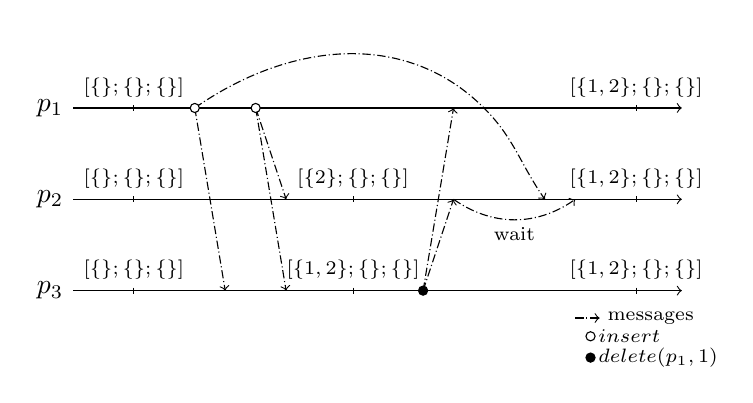
\begin{tikzpicture}[scale=1.1]
  
  \draw (-10pt,0pt) node[anchor=east]{$p_1$};
  \draw (-10pt,-30pt) node[anchor=east]{$p_2$};
  \draw (-10pt,-60pt) node[anchor=east]{$p_3$};

  \draw[->] (-10pt,0pt) -- (190pt,0pt);
  \draw[->] (-10pt,-30pt) -- (190pt,-30pt);
  \draw[->] (-10pt,-60pt) -- (190pt,-60pt);

  \scriptsize
  \draw (10pt,1pt) node[anchor=south]{[$\{\};\{\};\{\}]$} --
  (10pt,-1pt);
  \draw (10pt,-29pt) node[anchor=south]{[$\{\};\{\};\{\}]$} --
  (10pt,-31pt);
  \draw (10pt,-59pt) node[anchor=south]{[$\{\};\{\};\{\}]$} --
  (10pt,-61pt);

  \draw[->,densely dashdotted] (30pt,0pt) -- (40pt,-60pt);
  \draw[->,densely dashdotted] (50pt,0pt) -- (60pt,-30pt);
  \draw[->,densely dashdotted] (50pt,0pt) -- (60pt,-60pt);


  \draw (82pt,-29pt) node[anchor=south]{[$\{2\};\{\};\{\}]$} --
  (82pt,-31pt);
  \draw (82pt,-59pt) node[anchor=south]{[$\{1,2\};\{\};\{\}]$} --
  (82pt,-61pt);

  \draw [->,densely dashdotted] (30pt,0pt) to[out=35,in=135] (125pt,0pt)
  to[out=-45,in=125] (145pt,-30pt);

  \draw[fill=white] (30pt,0pt) circle (1.5pt);
  \draw[fill=white] (50pt,0pt) circle (1.5pt);

  \draw[->,densely dashdotted] (105pt,-60pt)--(115pt,-30pt);
  \draw[->,densely dashdotted] (105pt,-60pt)--(115pt,0pt);

  \draw[fill=black] (105pt,-60pt) circle (1.5pt);
  
  \draw[->,densely dashdotted]
  (115pt,-30pt)to[out=-35,in=-145]node[anchor=north]{wait}(155pt,-30pt);


  \draw (175pt,1pt) node[anchor=south]{$[\{1,2\};\{\};\{\}]$}-- (175pt,-1pt);
  \draw (175pt,-29pt) node[anchor=south]{$[\{1,2\};\{\};\{\}]$}--(175pt,-31pt);
  \draw (175pt,-59pt) node[anchor=south]{$[\{1,2\};\{\};\{\}]$}--(175pt,-61pt);
  
  \draw[->,densely dashdotted] (155pt,-69pt) -- (163pt,-69pt)
  node[anchor=west]{messages};
  \draw[fill=white] (160pt,-75pt)node[anchor=west]{$insert$}circle (1.5pt);
  \draw[fill=black] (160pt,-82pt)
  node[anchor=west]{$delete(p_1,1)$} circle (1.5pt);

\end{tikzpicture}

    \caption{\label{fig:timeline} Causality tracking example.}
  \end{figure}

  Figure~\ref{fig:timeline} depicts an editing session involving 3 users. The
  version vector with exceptions starts empty. Member $m_1$ inserts two
  characters in its document and broadcasts the corresponding messages. Member
  $m_3$ quickly receives both operations. Since it did not receive these
  operations before, and since they do not depend of any other operation, it
  integrates the operation identifiers to its causality structure. It also
  delivers the operation to the shared sequence structure
  (cf. Section~\ref{subsec:sequence}). In the meantime, Member $m_2$ only
  receives the second operation. Consequently, it marks the first operation of
  $m_1$ as exception and still integrates the received operation. Then, $m_3$
  removes the first character inserted by $m_1$ and broadcasts it. While $m_1$
  delivers the removal immediately, $m_2$ waits since the targeted operation
  belongs to the exceptions. Once it receives the missing first operation of
  $m_1$, the exception disappears and the delete operation is performed.

  The local upper-bound on space complexity is:
  \begin{equation}
    \mathcal{O}(|\mathcal{W}|)
  \end{equation}
  where $|\mathcal{W}|$ is the number of writers, i.e., users who modified the
  document at least once.  Such structure only requires to piggyback the
  identifiers of operation. Hence, the upper-bound on communication complexity
  is:
  \begin{equation}
    \mathcal{O}(o.\ln |\mathcal{R}|)
  \end{equation}
  where $o$ is the operation size determined by the shared sequence structure
  (cf. Section~\ref{subsec:sequence}), and the rest is determined by the
  communication layer (cf. Section~\ref{subsec:communication}).
  
\item [The anti-entropy protocol] periodically checks if the local replica
  diverges from another neighbor's one at random. It aims to retrieve missing
  operations that could have been lost during transmissions. For this purpose, a
  simple difference between vectors suffices.

  For instance, in the prior example depicted by Figure~\ref{fig:timeline},
  Member $m_2$ receives the second operation of $m_1$ before its first. To catch
  up, $m_2$ could send its version vector with exceptions to one of its
  neighbors chosen at random. Assuming that it picks $m_3$, the latter detects
  that, compared to its own vector, the remote member missed the first operation
  of $m_1$. Then, it sends it back to $m_2$ along with its own vector. Finally,
  $m_2$ follows the normal process for the received operations, and additionnaly
  merges its vector with the received one.

  Such protocol does not require any additional local metadata. However, the
  communication cost is prohibitively high which encourages to perform this
  reconciliation protocol with great care:
  \begin{equation}
    \mathcal{O}(|\mathcal{W}|+|\mathcal{W}|+x.o)
  \end{equation}
  where the first $|\mathcal{W}|$ designates the vector contained in the
  initiating message, and $|\mathcal{W}|+x.o$ the response to this message where
  $x.o$ are the missing operations.
\end{asparadesc}

\subsection{Shared sequence}
\label{subsec:sequence}

To guarantee eventually consistent~\cite{bailis2013eventual} replicas of the
shared document, \CRATE uses a conflict-free replicated data type for
sequences~\cite{shapiro2011comprehensive, shapiro2011conflict} with the
allocation function \LSEQ~\cite{nedelec2013concurrency, nedelec2013lseq} for its
unique and immutable identifiers.

\LSEQ stands for polyLogarithmic identifier allocator for SEQuences. It
allocates identifiers the size of which is polylogarithmically upper-bounded
(compared to the document size) and determined at generation (unique and
immutable). Thus, each identifier comprises a path and a globally unique marker
called disambiguator. We note the former as a list [$p_1.p_2\ldots p_k$] where
$p_k$ belongs to Integers. The union of paths produces a tree. For instance, the
factorization of paths [$13.37$] and [$13.42$] produces a tree where the element
$13$ has two children: $37$ and $42$. The challenge consists in keeping the
identifiers size growth under a sub-linear upper-bound on space complexity. The
rest of this section reviews \LSEQ's internal components and provides its
complexity analysis.

\begin{asparadesc}
\item [Two sub-allocation functions] with antagonist objectives allow \LSEQ to
  be independent of the application. Indeed, the editing behavior of users is
  unpredictable, i.e., get the \emph{a priori} knowledge of where and in which
  order the operations will be performed is impossible. Hence, instead of
  characterizing the editing behaviors of users with complex machine learning,
  \LSEQ uses two sub-allocation functions designed to handle trivial editing
  sequences, knowingly left-to-right editing and right-to-left editing. It
  assumes that the editing behavior is either one of these two, or a composition
  of them.

  We refer to left-to-right and right-to-left editing as monotonic editing since
  they come from the repeated insertions of characters at an adjacent position of
  the previously inserted one.
  
  The allocation functions allocate paths in order to save allocation space for
  the upcoming operations. In that spirit, the function designed for
  left-to-right editing allocates paths close of the leftmost available path.
  Thus, when new characters arrive, presumably at the right of the lastly
  inserted character, the allocation function still has a large number of
  available paths. Hence it does not need to increase the depth of the tree.

  For instance, assuming a 10-ary tree, a left-to-right allocation function, and
  a user writing QWERTY starting from Q to Y. When Character Q arrives,
  the function allocates a path in [$\mathbb{N}_{<10}$]. To leave available
  paths for future insertions, the function allocates a path close of the bound
  [$0$]. In this example, the resulting path is [$2$]. Then, Character W
  arrives, the functions allocates a path between Q's path [$2$], and the
  virtual boundary [$10$]. Once again, it chooses a path close of the previous
  path. It results in the path [$5$]. Incrementally, we obtain paths [$6$],
  [$7$], [$9$] for E R T, respectively. When Character Y arrives, there is no
  room for another path of size 1. Consequently, the depth of the tree increases
  to receive the new path allocated in [$9.\mathbb{N}_{<10}$]. Identically to
  prior insertions, the path is allocated close of the previous bound which is
  [$9.0$], resulting in [$9.1$].

  Nevertheless, this allocation strategy is not sufficient to handle any editing
  behavior. When the assumption of left-to-right editing does not hold,
  performance can be dramatically impacted.

  For instance, assuming a 10-ary, a left-to-right allocation function, and a
  user writing QWERTY starting from Y to Q. As for the prior example, the
  function allocates [$2$] for Y. When T arrives, it allocates a path between
  [$0$] and [$2$] resulting in the path [$1$]. When R arrives, the tree has no
  room for a new path at depth 1. As consequence, the path is allocated in
  [$0.\mathbb{N}_{<10}$]. Since it keeps allocating paths close from the
  previous bound, the resulting path is [$0.1$]. When E arrives, the tree must
  grow again etc.

  Each sub-allocation function is application dependent.  \LSEQ uses two
  antagonist strategies to adapt to any editing behavior. 

\item [A hash function] chooses among the two sub-allocation functions. The
  choice is made randomly following a uniform distribution. As such, it does not
  favor any editing behavior and provides the independence of the allocation
  function from any editing behavior.

  Using antagonist sub-allocation functions forces all peers to make identical
  choices~\cite{nedelec2013concurrency}. To reach that goal, they all use a
  similar hash function initialized with a common seed and shared within the
  document. When a user inserts a new element in the sequence, \LSEQ firstly
  processes the depth of the new path, and secondly defers the allocation to the
  function designated by the hash of the depth.

\item [An exponential tree]~\cite{andersson1996faster, andersson2007dynamic}
  represents the shared document. Such tree has the particularity that each
  element has twice as much children as its parent.  Hence, paths are sequence
  of numbers where each concatenation belongs to a subset of Integer the size of
  which doubles compared to the prior concatenation. For instance, if a path of
  size 1 is chosen among [$\mathbb{N}_{<32}$], a path of size 2 is chosen among
  [$\mathbb{N}_{<32}.\mathbb{N}_{<64}$] etc.

  An exponential tree with a root of maximum arity $r$ has paths of size $k$
  chosen among [$\mathbb{N}_{<r}.\mathbb{N}_{<2r}\ldots\mathbb{N}_{<2^{k-1}r}$].
  Due to the subsets growth, the binary representation of paths requires one
  additional bit to encode each concatenation. For instance, a path chosen among
  [$\mathbb{N}_{<32}$] is encoded on $log_2(32)=5$ bits, a path chosen among
  [$\mathbb{N}_{<32}.\mathbb{N}_{<64}$] is encoded on $log_2(32)+log_2(64)=11$
  bits, etc.
  
  An exponential tree with a root of maximum arity $r$ has paths of size $k$
  encoded on:
  \begin{equation}
    \sum\limits_{i=0}^{k-1}(\log_2(r)+i) =k^2+(log_2(r)-{1\over{2}})k =
    \mathcal{O}(k^2) \,\, bits
  \end{equation}

  A balanced exponential tree reaching a depth $k$ (i.e., all its branches are
  filled) holds uptill:
  \begin{equation}
    \sum\limits_{i=1}^{k} {2^{(i^2+i)/2}} \,\, elements
  \end{equation}

  An exponential tree reaching a depth $k$ with only one branch filled per level
  holds uptill:
  \begin{equation}
    2^{k+1}-2 \,\, elements
  \end{equation}

  An exponential tree reaching a depth $k$ with only one element per level
  (worst case) holds uptill: 
  \begin{equation}
    k \,\, elements
  \end{equation}

  \begin{table}
    \centering
    
\begin{tabularx}{0.6\textwidth}{@{}Xcc@{}}

  \toprule
  \textsc{Editing behavior} & \multicolumn{2}{c}{\textsc{Space}} \\ \cmidrule{2-3} 
                   & \textsc{Identifier} & \textsc{Sequence} \\ \midrule
  Random editing & $\mathcal{O}(\log I)$ & $\mathcal{O}(I\log I)$ \\
  Monotonic editing & $\mathcal{O}((\log I)^2)$ & $\mathcal{O}(I \log I)$ \\
  Worst case & $\mathcal{O}(I^2)$ & $\mathcal{O}(I^2)$ \\ \bottomrule
\end{tabularx}

    \caption{\label{table:lseqspace}
      Upper-bound on space complexity of \LSEQ. Where $I$ is the document size.}
  \end{table}
  
  From this counting, we deduce the space complexity of
  \LSEQ. Table~\ref{table:lseqspace} shows both the space complexity of each
  identifier and the space complexity of whole tree structure representing the
  sequence. When the tree is balanced, its depth is upper-bounded by
  $\mathcal{O}(\sqrt{\log I})$. Since the identifier encoding grows
  quadratically compared to the depth of the tree, it results in
  $\mathcal{O}(\log I)$. From the same reasoning, the identifiers of monotonic
  editing are polylogarithmic. In the worst case, where the tree has one element
  per level, identifiers grows quadratically. When the tree structure factorizes
  identifiers, it results in $\mathcal{O}(I\log I)$ since each element holds a
  single concatenation of the path the size of which grows logarithmically.  In
  the the worst case, the last identifiers contains the full tree, hence,
  $\mathcal{O}(I^2)$.
  
  An alphabetical order maintains a dense total order among elements. It uses
  both the path and disambiguators of the identifier. While the former aims to
  give a fast and easy way to create and order elements relatively from each
  other. The objective of the latter is twofold:
  \begin{inparaenum}[(i)]
  \item to order concurrent operations that happen to have an identical path and
  \item to allow the allocation of new identifiers in-between them.
  \end{inparaenum}

  For instance, let [$3$] be the path of Element Q inserted by Member $m_x$, and let
  [$4$] the path of Element T inserted by Member $m_y$. When a member $m_1$ inserts W
  between those elements, the depth of the tree must grow to welcome the new
  element. Assuming that depth 1 has a maximum arity of 8, the identifier is
  allocated in the range from [$3.0$] to [$3.15$].  In this example, the resulting
  path is [$3.6$]. In the meantime, another member $m_2$ inserts R between Q and T
  which happens to result in the path [$3.6$] too. To ensure a total order,
  disambiguators are associated with each path composed of a monotonically
  growing counter and a globally unique site identifier. Here, the identifier of
  Element W is composed of the path [$3.6$] and disambiguator
  [$\langle m_x,\,1\rangle$, $\langle m_1,\,1\rangle$] and the Element R is composed of
  the path [$3.6$] and disambiguator [$\langle m_x,\,1\rangle$,
  $\langle m_2,\,1\rangle$].  The comparison starts to examine the first
  concatenations which are equal.  Then, the comparison concerns the path of the
  second level of the tree which are equals too. Hence, it examines the
  disambiguators to determine that W is located before R because $m_x < m_y$ in
  this case. The resulting sequence is QWRT.  
\end{asparadesc}

\begin{table}
  \centering
  
\begin{tabularx}{0.455\textwidth}{@{}Xcccc@{}}
  \toprule
  \textsc{Editing} & \multicolumn{4}{c}{\textsc{Time}} \\
  \textsc{behavior} & \multicolumn{2}{c}{\textsc{Local}} & \multicolumn{2}{c}{\textsc{Remote}} \\ \cmidrule(r){2-3} \cmidrule(l){4-5}
  & \textsc{ins} & \textsc{del} & \ \ \ \ \textsc{ins} & \textsc{del}  \\ \midrule
  Random & $\mathcal{O}(\sqrt{\log I})$ & $\mathcal{O}(1)$ & \multicolumn{2}{c}{$\mathcal{O}(\log I + \sqrt{\log I})$} \\
  Monotonic & $\mathcal{O}(\log I)$ & $\mathcal{O}(1)$ & \multicolumn{2}{c}{$\mathcal{O}((\log I)^2 +\log I)$} \\
  Worst case & $\mathcal{O}(I)$ & $\mathcal{O}(1)$ & \multicolumn{2}{c}{$\mathcal{O}(I)$} \\ \bottomrule
\end{tabularx}


  \caption{\label{table:lseqtime}
    Upper-bound on time complexity of \LSEQ. Where $I$ is the document size.}
\end{table}

Table~\ref{table:lseqtime} shows the time complexity of operations of \LSEQ
divided between the local and remote parts of the optimistic replication. The
local insertion is in charge of allocating an identifier. Since, the balanced
tree resulting from random editing reaches a depth of
$\mathcal{O}(\sqrt{log I})$ and requires as much comparisons to create the new
identifiers. When they are integrated, it requires as much binary searches to
locate their correct position. A tree filled by monotonic editing grows
logarithmically. Hence, the time complexity upper-bound is higher than the
balanced structure. Finally, the worst case requires to consider the path of
each element to create the new identifiers. Then, at integration, it requires
one comparison per level (i.e. per element) to find its location. The local
delete operation is only in charge of broadcasting the identifier to all
participants, hence, the constant time complexity.

% \TODO{To summarizes, the space complexity analysis reveals that the allocation
% function \LSEQ sacrifices on the worst-case space complexity to improve the
% space complexity of the monotonic editing behaviors. Nevertheless, in text
% editing, the worst-case happens with a very low probability compared the other
% cases. Furthermore, it is worth noting that usually, the authors do not write a
% document in a single round, starting from the beginning to go straight up to
% the end (as the monotonic analysis could suggest). On the contrary, the authors
% write sections, structure the documents, perform corrections, rewrite parts of
% the document, reorganize, etc. This behavior (between random and monotonic
% behavior) tends to even up the branches of the underlying tree of \LSEQ. In
% the case of random editing, the space complexity is asymptotically optimal
% $O(log\,n)$ while it is very interesting in a "normal setting" $O((log\,n)^2)$.}

\begin{figure*}
  \centering
  \subfloat {\input{input/lseqtreeexampleA.tex}}
  \hspace{10pt}
  \subfloat {\input{input/lseqtreeexampleB.tex}}
  \caption{\label{fig:lseqtreeexample}\LSEQ tree handling two monotonic
    editing behaviors.}
\end{figure*}


\begin{asparadesc}
\item [As summary,] Figure~\ref{fig:lseqtreeexample} depicts the functioning of
  \LSEQ resulting in two trees after scenarios creating the sequence $QWERTY$:
  \begin{inparaenum}[(i)] 
  \item the left-to-right editing sequence [($Q,\,0$), ($W,\,1$), \ldots] and
  \item the right-to-left editing sequence [($Y,\,0$), ($T,\,0$), \ldots].
  \end{inparaenum}
  In both cases, the exponential tree of \LSEQ starts with an arity $32$ and
  doubles it at each level. It uses the $frontEditing$ and $endEditing$
  sub-allocation functions which are sub-allocation functions designed for
  right-to-left and left-to-right monotonic editing behaviors. The hash function
  designates the $frontEditing$ sub-allocation function to the first level of
  the tree, and the $endEditing$ sub-allocation function to the second
  level. Since the first level of the tree uses the function $endEditing$, the
  scenario involving the left-to-right editing sequence results in a tree of
  depth 1. On the other hand, the antagonist scenario shows \LSEQ identifiers
  that quickly reach a level of the tree where the sub-allocation function is
  designed to handle the right-to-left editing behavior.
\end{asparadesc}

\subsection{Graphical user interface}

To perform their changes on the shared document, users have a visual
representation of their respective local copy in their web browser.  \CRATE
provides a look-up function to gets the identifier at the index, and. It gets
the identifiers at a designated index, and converse. Thus, when users perform
their insertions, \CRATE gets the identifiers at the targeted position and
generates the new identifier. When it receives an identifier, it firstly inserts
it into the tree structure and secondly get its index to notify the view.

\begin{table}
  \centering
  
\begin{tabularx}{0.6\textwidth}{@{}Xc@{}}
  \toprule
  \small
  \textsc{Editing behavior} & \textsc{Time} \\
  & \ \ \ \ \ \ \ \ \ \textsc{lookup} \ \ \ \ \ \ \ \ \ \\ \midrule
  Random editing & $\mathcal{O}(2^{\sqrt{\log I}})$ \\
  Monotonic editing / Worst case & $\mathcal{O}(I)$ \\ \bottomrule
%%  Worst case & $\mathcal{O}(I)$ \\ \bottomrule
\end{tabularx}


  \caption{\label{table:lseqlookup}
    Upper-bound on time complexity of the look-up on a \LSEQ structure.
    Where $I$ is the document size.}
\end{table}

Each element in the tree keeps track of its number of children. Such information
allows quick withdrawing of ranges of elements. Table~\ref{table:lseqlookup}
shows the time complexity of the look-up operation. When the tree structure is
balanced, only a small fraction of the tree need to be browsed to find the index
of elements. On the other hand, the structure generated by monotonic editing
leads to a linear look-up. Fortunately, the latter case does not happen at local
insertions since \CRATE can lazily store the last generated identifier to create
the new one. If a user starts to edit each time at different positions, the
structure starts to be balanced, and the look-up becomes more efficient
relatively to the document size. Upon reception, since users only have a partial
view of the whole document, the look-up of the received operation may fall into
a range of element not loaded by the view.

%%% Local Variables: 
%%% mode: latex
%%% TeX-master: "../paper"
%%% End: 
